\section{Системное проектирование}
\label{sec:arch}

После тщательного изучения предметной области, постановки целей и выделения задач дипломного проектирования, была
разработана структурная схема системы функционального контроля ТС КМУ артиллерийского дивизиона.
Система разделена на несколько слабо связанных модулей.
Данная система представляет собой клиент серверную архитектуру~\cite{cl_s},
где АРМ является сервером и осуществляет проверку клиентов -- подключенных устройств.

\begin{figure}[ht]
	\centering
	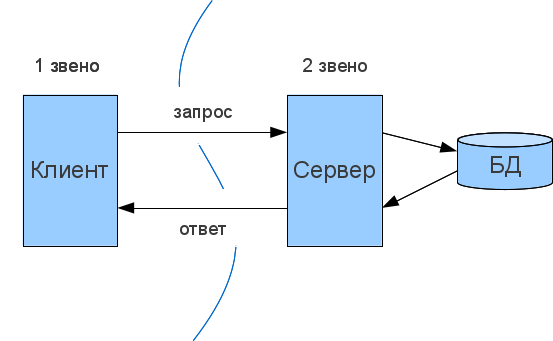
\includegraphics[scale=1.1]{client-s}
	\caption{Архитектура клиент-сервер~\cite{cl_s}}
	\label{fig:sec_arch:client}
\end{figure}

В системе имеются следующие блоки:
\begin{itemize}
	\item управляющий модуль
	\item блок тестирования и настройки ЛВС
	\item блок тестирования метеокомплекта
	\item блок тестирования навигационной системы
	\item блок автоматизации обнаружения устройств
	\item блок тестирования радиоканалов
	\item блок тестирования специального принтера
\end{itemize}

Данные модули являются довольно независимыми друг от друга. Из-за того, что системы тестирует множество различных
устройств, модули, работающие с периферийными устройствами имеют связь лишь с управляющим модулем.

Структурная схема, с изображением всех блоков и связей между ними, приведена на чертеже ГУИР.400201.065 С1.

Рассмотрим подробнее функциональные блоки системы.

\textit{Управляющий модуль} занимается обменом данными с остальными модулями, он занимается посылкой команд
тестирования, приемом и выводом информации от модулей, работающих с периферией. Также данный модуль отвечает за общение
с пользователем программы и обработкой поступающих от устройств диагностических данных.

Данный модуль общается с другими путем вызова публично доступных методов других модулей. Управляющий модуль может также
передавать данные и внешним модулям, посредством доступного и удобного API. Данный способ может быть полезен при
включении системы функционального контроля в более крупную, например, таковой системой является комплекс автоматизации
КМУ артиллерийского дивизиона.

Взаимодействие с пользователем осуществляется с помощью графического интерфейса, основанного на Qt виджетах. Передача
управления другим блокам осуществляется с помощью команд контекстного меню и кнопок графического интерфейса.

Управляющий блок позволяет:
\begin{itemize}
	\item взаимодействовать с блоком тестирования и настройки ЛВС
	\item взаимодействовать с блоком тестирования метеокомплекта
	\item получать доступ к функциям тестирования специального принтера
	\item осуществлять доступ к системе автообнаружения устройств
	\item получать доступ к модулю тестирования радиоканалов
	\item осуществлять тестирование системы навигации, путем взаимодействия с соответствующим модулем
	\item осуществлять логгирование событий и вывод статистики
	\item проводить контроль доступа к подсистемам функционального контроля
\end{itemize}

\textit{Блок управления пользовательским интерфейсом} отвечает за взаимодействие с пользователем с помощью средств Qt.
Блок управляет содержанием и поведением окон приложения.

\textit{Блок автоматизации обнаружения устройств} занимается обнаружением всех подключенных к системе устройств,
настройку параметров общения с ними, ведение списка подключенной периферии.

Данный блок имеет крайне важное значение в связи с тем, что до недавнего времени операторам АРМ приходилось настраивать
все подключенные устройства вручную.
Сложнее всего -- идентифицировать правильно подключенные к АРМ устройства, так как
зачастую они подключены через COM порты и имеют в системе практически идентичные названия(TTYS0, TTYS1 и т.д).

Данный блок имеет следующие составляющие:
\begin{itemize}
		\item библиотека доступных протоколов
		\item модуль сканирования подключенных устройств
		\item модуль идентификации подключенных устройств
		\item внешний интерфейс для добавления новых устройств в библиотеку. Предоставляет возможность расширения библиотеки протоколов.
		\item модуль настройки подключенных устройств
		\item модуль ведения отчетности о подключенных устройствах
\end{itemize}

Данный модуль обращается к библиотеке устройств(протоколов) и производит поиск данных устройств в системе.

При дальнейшем развитии проекта предполагает интерес вынесения функционала данного блока в область ядра ОС. К сожалению,
данный подход имеет сложности в виду необходимости предоставления исходных кодов вместе с продуктом, в связи с
требованиями лицензии GPL.

Блок автоматизации обнаружения устройств не производит тестирование и диагностику подключенных ТС. Данный модуль лишь
помогает установить требуемые параметры для общения согласно заданному протоколу\break(проверка четности, скорость передачи и
т.п.).

\textit{Блок тестирования специального принтера} осуществляет проверку работоспособности принтера экипажа. Данный модуль
позволяет проверить состояние принтера, проверить уровень чернил и настройку параметров печати путем оправки тестовой
страницы на печать.

\textit{Блок тестирования и настройки ЛВС} позволяет:
\begin{itemize}
	\item настроить ip адреса, используемые программой для общения к внешним устройствам, к другим машинам в
		ЛВС
	\item провести проверку работоспособности сети
	\item собирать различную диагностическую информацию о состоянии сети: процент потерянных
		пакетов, время отклика между узлами ЛВС
	\item вести статистику, используя полученные данные
	\item выводить полученные результаты на экран монитора, либо на печать
\end{itemize}

Все АРМ внутри КМУ подключены к ЛВС, также к сети подключены и такие устройства как радиостанции и некоторые датчики,
обменивающиеся информацией с АРМ с помощью протоколов стека TCP/IP.
Машина управления также может связаться с другими машинами комплекса, используя ЛВС.

\textit{Блок тестирования навигационной системы} позволяет провести функциональный контроль подключенных к АРМ устройств
навигации.

Комплексная навигационная система состоит из следующих устройств:
\begin{itemize}
	\item бесплатформенная навигационная система(БИНС)
	\item блок измерительный спутниковый (БИС)
	\item датчик пути цифровой(ДПЦ)
\end{itemize}

Напрямую система общается лишь с БИНС. Обмен информацией с БИС и ДПЦ идет через БИНС.
Данные устройства позволяют получать различную информацию о местоположении машины, получать информацию о наклоне
машины относительно плоскостей координат(крен, тангаж).

Информация с данных датчиков отображается на экран монитора, печатается на принтере либо сохраняется в файл для
дальнейшей обработки. Система имеет множество различных регистров, хранящих данные о скорости машины, пройденном пути и
т.п. Необходимо проверить доступность данной информации, верифицировать ее достоверность.

Данная система также может работать с системами GPS и GLONASS, поэтому также следует проверять следующие моменты:
\begin{itemize}
	\item доступность спутников
	\item величину сигнала со спутника
	\item автоматический поиск спутников
	\item верность полученной информации
	\item одновременное использование обеих систем навигации
	\item переключение на другую систему ввиду слабого или отсутствующего сигнала спутника
\end{itemize}

Используя имеющиеся датчики, КНС может получать данные о местоположении даже ввиду отсутствия GPS/GLONASS спутников в
зоне досягаемости.
Это достигается за счет использования одометров, гироскопов, акселерометров. Обработкой этих данных
занимается БИНС.
Поэтому необходимо также проверить правильность работы самого БИНС.

\textit{Блок тестирования радиоканалов} занимается тестированием и настройкой средств радиосвязи.

В машинах КМУ установлено несколько различных типов раций, общение с которыми имеет определенные отличия.
Рации имеют
различный тип внутреннего устройства, различный форм фактор, различный диапазон для передачи данных.

Общение через радиоканал может осуществляться как внутри машины, так и с другими машинами и объектами на местности.
Блок тестирования радиоканала позволяет проверить работу различных типов раций во всевозможных режимах работы.

Например, рация в КМУ может иметь следующие режимы работы:
\begin{itemize}
		\item общение точка-точка внутри машины
		\item режим конференц связи внутри машины
		\item режим общения с членом экипажа другой машины
\end{itemize}

В связи с данными сложностями, необходимо проверить следующие варианты работы системы:
\begin{itemize}
	\item работа в режиме точка-точка внутри машины
	\item возможность осуществления конференц связи
	\item проверка работы зашифрованного обмена
	\item обмен данными по радиоканалу
	\item возможность связи с другими машинами КМУ
	\item возможность обмена на всем спектре доступных частот
\end{itemize}

\textit{Блок тестирования метеокомплекта} позволяет проводить тестирование работы метеокомплекта, который имеется во
всех КМУ.

Метеокомплект предоставляет следующую информацию:
\begin{itemize}
	\item осадки
	\item атмосферное давление
	\item температура
	\item относительная влажность
	\item направление ветра
	\item скорость ветра
\end{itemize}

Необходимо проверить доступность всей вышеприведенной информации, проверить ее достоверность, провести настройку
устройства.

